
\begin{figure}[H]
\centering
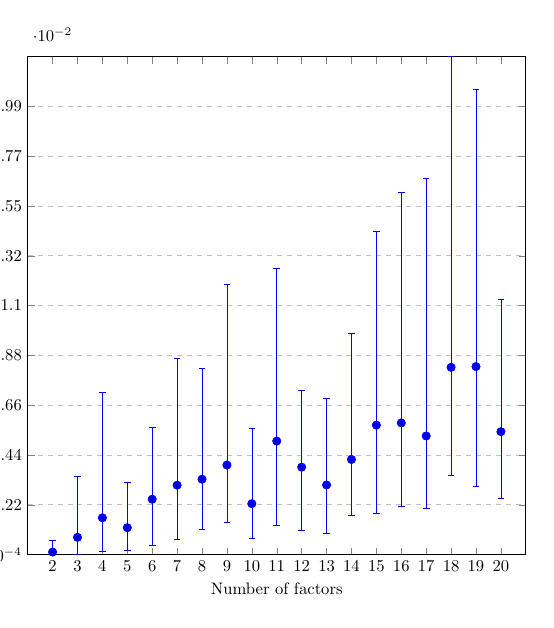
\begin{tikzpicture}[scale=0.6, trim axis left, trim axis right]
\begin{axis}[
    width=1\textwidth,
    height=1\textwidth,
    xlabel={Number of factors},
    ylabel={Time taken (s)},
    xmin=1.0, xmax=21.0,
    ymin=4e-06, ymax=0.022079,
    xticklabels={2, 3, 4, 5, 6, 7, 8, 9, 10, 11, 12, 13, 14, 15, 16, 17, 18, 19, 20},
    xtick={2, 3, 4, 5, 6, 7, 8, 9, 10, 11, 12, 13, 14, 15, 16, 17, 18, 19, 20},
    ytick={4e-06, 0.0022115, 0.004419, 0.0066265, 0.008834, 0.0110415, 0.013249, 0.0154565, 0.017664, 0.0198715},
    ymajorgrids=true,
    grid style=dashed,
]

\addplot+[
    blue,
    very thick,
    forget plot,
    only marks
    ]
    plot[
    very thick,
    error bars/.cd,
    y dir=plus,
    y explicit
    ]
    table[x=x,y=y,y error expr=\thisrow{y-max}] {
    x    y    y-max
    11	0.0050348625	0.0076751375
10	0.0022605625	0.0033444375
13	0.0030904875	0.0038565125
12	0.00387965	0.00338435
15	0.0057422625	0.0086097375
14	0.004221375	0.005607625
17	0.00526105	0.01139895
16	0.005837375	0.010202625
19	0.0083349	0.0122971
18	0.00830305	0.01377595
20	0.0054513125	0.0058676875
3	0.000769125	0.002685875
2	0.000117275	0.000506725
5	0.00119695	0.00202105
4	0.0016340375	0.0055409625
7	0.0030799625	0.0056330375
6	0.002458725	0.003203275
9	0.0039727375	0.0079962625
8	0.003345775	0.004911225

    };

\addplot+[
    blue,
    very thick,
    forget plot,
    only marks
    ]
    plot[
    very thick,
    error bars/.cd,
    y dir=plus,
    y explicit
    ]
    table[x=x,y=y,y error expr=\thisrow{y-min}] {
    x    y    y-min
    11	0.0050348625	-0.0037238625
10	0.0022605625	-0.0015505625
13	0.0030904875	-0.0021564875
12	0.00387965	-0.00278665
15	0.0057422625	-0.0039052625
14	0.004221375	-0.002456375
17	0.00526105	-0.00319205
16	0.005837375	-0.003690375
19	0.0083349	-0.0053079
18	0.00830305	-0.00477605
20	0.0054513125	-0.0029693125
3	0.000769125	-0.000737125
2	0.000117275	-0.000113275
5	0.00119695	-0.00101795
4	0.0016340375	-0.0015070375
7	0.0030799625	-0.0023959625
6	0.002458725	-0.002035725
9	0.0039727375	-0.0025607375
8	0.003345775	-0.002208775

    };

\end{axis}
\end{tikzpicture}
\vspace{-0.3cm}
\caption{Small primes, Iterations: 1 }\label{fig:LenstrasEllipticCurveFactorizationsmallprimes(maximumIterations:1)factors}
\end{figure}
